\section{convnets}

\begin{frame}
	\frametitle{Convolutional Neural Networks (CNN)}

	\begin{columns}
       		\column{0.5\textwidth}
      		\begin{figure}
             		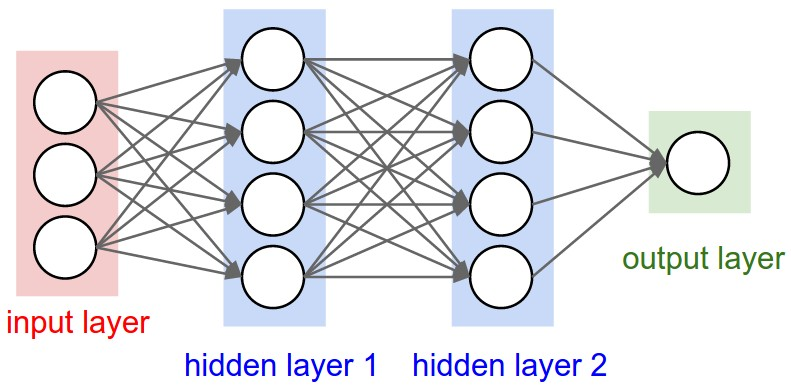
\includegraphics[width=1\textwidth]{Pics/neural_net2}
                \end{figure}
                \column{0.5\textwidth}
                \begin{figure}
                        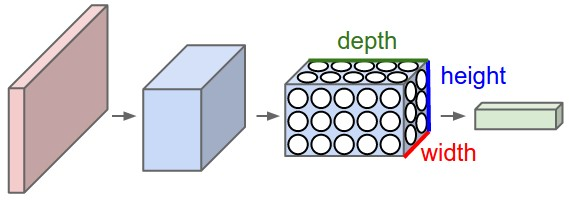
\includegraphics[width=1\textwidth]{Pics/cnn}
                \end{figure}

        \end{columns}

	\vskip 0.5cm

	A CNN arranges its neurons in three dimensions (width, height, depth). 
	Every layer of a CNN transforms the 3D input volume to a 3D output volume of neuron activations.
	Neurons in a layer are connected only to a small region of the layer before it.

\end{frame}


\begin{frame}
	\frametitle{CNN architecture}

	\begin{itemize}
		\item Convolutional Layer
		\item Pooling Layer
		\item Fully-Connected Layer
	\end{itemize}

	We will stack these layers to form a full CNN architecture.

\end{frame}

\begin{frame}
	\frametitle{Convolutional layer}

	\begin{figure}
       		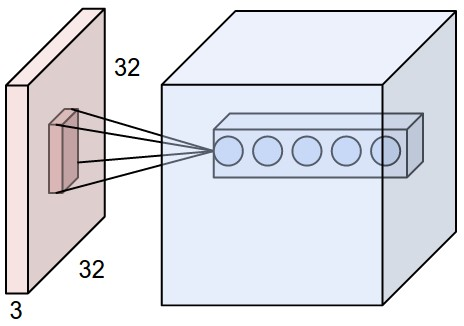
\includegraphics[width=0.4\textwidth]{Pics/depthcol}
      	\end{figure}

	Set of learnable filters which \textit{slides} across the width and height of the input volume.\\
	3 hyper-parameters: depth (nr of filters), stride, zero-padding.

\end{frame}

\begin{frame}
        \frametitle{Convolutional layer}

	\begin{itemize}
		\item Accepts a volume of size $W_1xH_1xD_1$
		\item Requires 4 parameters: number of filters $K$, their size $F$, the stride $S$, the amount of zero padding $P$
		\item Produces a volume of size $W_2xH_2xD_2$ where:
		\begin{itemize}
			\item $W_2 = (W_1 - F +2P)/S+1$
			\item $H_2 = (H_1 - F +2P)/S+1$
			\item $D_2 = K$
		\end{itemize}
	\end{itemize}

	Usually: $F=3$,$S=1$,$P=1$.

	Demo: \url{http://cs231n.github.io/convolutional-networks/}

\end{frame}

\begin{frame}
        \frametitle{Weights in filters}

        \begin{figure}
                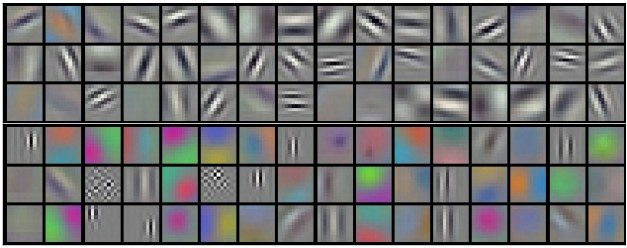
\includegraphics[width=0.9\textwidth]{Pics/weights}\\
		\small{Example filters learned by Krizhevsky et al. Each of the 96 filters shown here is of size [11x11x3], and each one is shared by the 55*55 neurons in one depth slice}
        \end{figure}

\end{frame}


\begin{frame}
        \frametitle{Pooling layer}

        \begin{columns}
                \column{0.5\textwidth}
                \begin{figure}
                        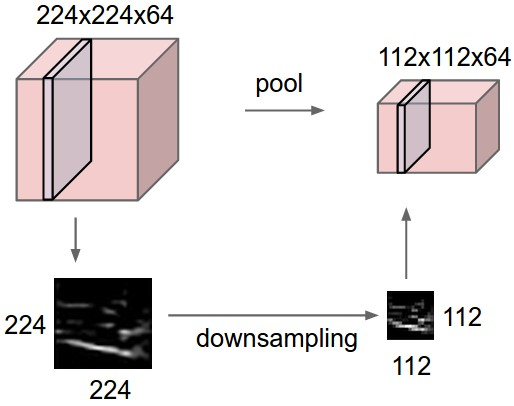
\includegraphics[width=1\textwidth]{Pics/pool}
                \end{figure}
                \column{0.5\textwidth}
                \begin{figure}
                        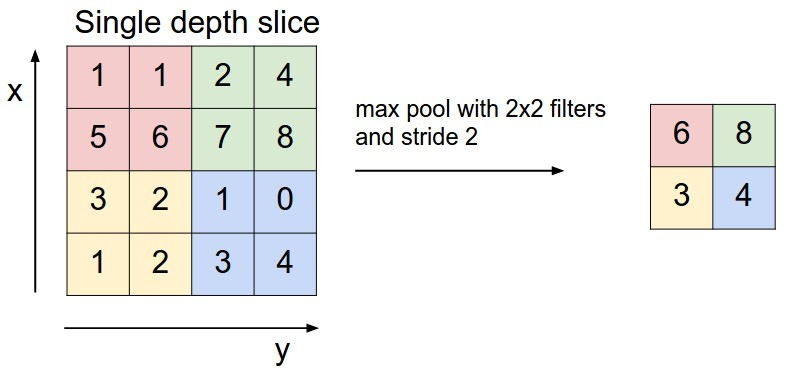
\includegraphics[width=1\textwidth]{Pics/maxpool}
                \end{figure}

        \end{columns}

	\vskip 0.5cm
	Size will influence the proportion of weights retained.

\end{frame}

\begin{frame}
	\frametitle{Layer patterns}

	INPUT $\rightarrow$ [[CONV $\rightarrow$ RELU]*N $\rightarrow$ POOL?]*M $\rightarrow$ [FC $\rightarrow$ 
	RELU]*K $\rightarrow$ FC

	\vskip 1cm

	More examples: \url{http://cs231n.github.io/convolutional-networks/}

\end{frame}

\begin{frame}
	\frametitle{Applications to biological data}

	From various sources:
	\begin{itemize}
		\item -omics (gen-, transcript-, epigen-, prote-, metabol-)
		\item bioimaging (cellular images, ...)
		\item medical images (clinical imaging)
		\item brain/body machine interfaces (ECG, EEG, ...)
	\end{itemize}

\end{frame}

\begin{frame}
        \frametitle{Applications to biological data}

	\begin{figure}
                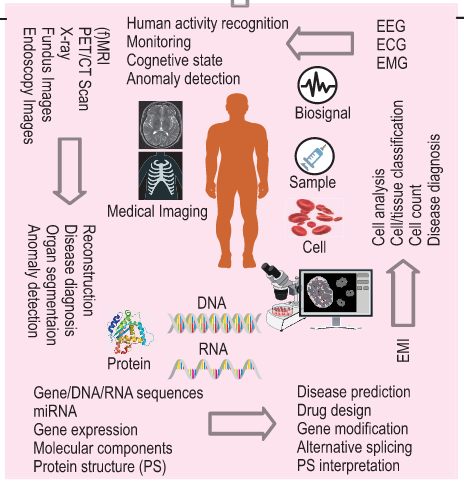
\includegraphics[width=0.6\textwidth]{Pics/biology.png}
        \end{figure}

\end{frame}

\begin{frame}
	\frametitle{Omics}

	Mining DNA/RNA sequence data to:
	\begin{itemize}
		\item identify splicing junction
		\item classify somatic point mutation-based cancer
		\item predict DNA- and RNA-binding motifs
		\item relate disease-associated variants to gene expression
		\item estimate DNA methylation patterns
		\item ...
	\end{itemize}

\end{frame}

\begin{frame}
	\frametitle{Splice junctions}

	\vskip 0.3cm
	Deep neural networs outperform other methods.

	\begin{figure}
                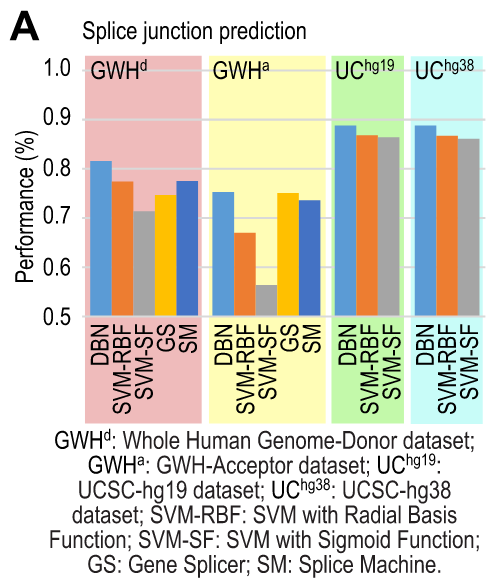
\includegraphics[width=0.45\textwidth]{Pics/splice.png}
        \end{figure}

\end{frame}

\begin{frame}
	\frametitle{Open issues}

	\begin{itemize}
		\item theory of deep learning is not completely understood making outcomes difficult to interpret
		\item susceptible to misclassification and overclassification
		\item uncertainty in building architectures
		\item bootstrapping not possible
	\end{itemize}

\end{frame}

\begin{frame}
        \frametitle{Future perspectives}

        \begin{itemize}
		\item improving theoretical foundations on the basis of experimental data
		\item assessment of model's computational complexity and learning efficiency
		\item novel data visualization tools
		\item in biology: reduce data redundancy and extract novel information
		\item \textit{ad hoc} computational infrastructures
	\end{itemize}

\end{frame}

\begin{frame}
        \frametitle{Wrap up}

        \begin{itemize}
                \item CNN arranges its neurons in three dimensions
                \item Different type of layers (convolution, pooling, ...)
                \item Weights in filters are learned
		\item Promising applications to biological data.
        \end{itemize}

\end{frame}








